% siminos/gudorf/thesis/chapter/trawl.tex
% $Author: predrag $ $Date: 2020-10-24 01:45:26 -0400 (Sat, 24 Oct 2020) $

%Possible figures
%initial conditions
%final resulting \twots\
%various twots
Once we have the ability to solve \refeq{e-kssFb} we need to first create a collection
of \twots. The only requirement that the collection must satisfy is that it must capture
all fundamental patterns by adequately sampling the set of \twots. In other words an exhaustive
search is not our aim; not only that, but also the collection need not sample all {\spt} domain sizes.
We hypothesize that there is some upper bound on the {\spt} size of fundamental tiles due to {\spt}
correlation lengths.

Once the collection is deemed sufficient we proceed to visual inspection. In this manner
we determine the most frequent patterns and single them out as tile candidates. This is
done by literally clipping them out of the \twots\ that they shadow. Each clipping is
then treated as an initial guess for a fundamental tile which is itself a \twot. Therefore,
these represent initial conditions for the optimization method. It is not a guarantee
that every clipping converges to a \twot; therefore the number of attempts to find a tile
should continue until it does in fact converge. The number of convergence attempts is typically
proportional to how confident we are that the pattern being scrutinized is in fact a tile.

Once a collection of tiles is collected, we can construct new and reproduce known \twots.
This is completed with a method we refer to as ``gluing''. It is as straightforward as one
might infer: tiles are combined in a {\spt} array to form initial conditions used to find larger
\twots. Methods of gluing temporal sequences of \twots\ exist but never has the ability to
glue \twots\ spatiotemporally existed before.

The numerical methods of \refsect{sect:adjointdescent} and
\refsect{sect:gaussnewton}, and \refsect{sect:gmres}
enable us survey the infinite \spt\ state space by
finding \twots\ which adequately sample the ensemble of
solutions
that solve \refeq{e-kssFb}.
This is possible provided we start with sufficiently good
initial guesses to solve for minimizers of \refeq{e-costfunctional},
where ``good'' initial conditions are any doubly periodic scalar fields
which converge to \twots\ via our numerical optimization.
To demonstrate the efficacy of our \spt\ methods we will
contrast them with conventional methods. Before this, however,
we will first comment on some philosophical differences between
the initial value problem and boundary value problem.
In \refsect{sect:variational} we describe the reformulation
of \refeq{e-ks} without going into much detail of the motivations
to do so. In what follows we hope to convince the reader that
the variational formulation truly is the only chance for studies
of nonlinear chaotic equations.
This body of work is critically dependent
on being able to find exact time invariant solutions of the \KSe.
What do we mean by this precisely?
The nature of the word ``exact'' which is present in many such
discussions (e.g. ``Exact Coherent Structures''\rf{WK04,W01,W02})
is actually rather nebulous..
In fact, the definition was never really meant as a descriptor
of data but rather it was a manner by which to categorize
fundamental solutions of the governing equations\rf{W01}.
We argue that in fact that describing solutions of
the dynamical systems as ``exact'' is disingenuous. In dynamical
systems there is always going to be propagation of error
due to time integration in the presence of a positive Lyapunov
exponent. We will only offer a qualitative description, as
finding bounds on the error in nonlinear dynamical systems
is a tough proposition and can only be done in certain cases\rf{DV01}.
For example, let us take time integration which produces a discrete
representation of a periodic orbit. Even in the best case
scenario where the initial condition yields a
recurrence within machine precision after one period
the trajectory will eventually escape due to magnification
of numerical errors. Other reason why we claim these trajectories
to not be exact is because they can not be reproduced (in a very
strict case, to be fair).
Unless there
is an actual exchange of data there is a zero percent likelyhood
that a time invariant solution will be reproduced exactly by
another computation. Why? Even in the best case scenario wherein the
numerical parameters are identical between the two computations,
the only manner in which the solutions would be exactly the same
is if the same exact initial condition within machine
precision was used with the exact same
numerical methods (we disregard the fact that
same computer would be required as well).
It is straightforward to use the same numerical procedure but
there is no manner by which to procure the same initial condition.
One might argue that this is too strict and the only demand
is that one be ``close enough''. The issue with this
is that this error distorts any further calculations that
may be desired. Once again
one can say that this is not an issue as long as the results are
``close enough'' within some metric but there may come a time
where these error bars compound to produce results that in fact
are not close enough. One such calculation is the linear stability
analysis of solutions. Small errors can have a profound effect
as the calculations are susceptible to numerical overflow and
numerical underflow (numbers getting too large or small, respectively).
We argue that just as one wants to find
quantities which are \textit{topologically invariant} (independent
of coordinate system) we also would
like it to be \textit{numerically invariant}
(independent of numerical method). As we have attempted
to describe, we believe this is a hopeless endeavor
for the initial value problem
but in the context of our \spt\ differential algebraic equations
this is very possible up to the smallest of differences
(machine precision). One might think that the same arguments
apply, but because there is no longer any dynamics we do not
run into the same issues. The reason for this discrepancy is
due to the differing forms of the equations. The differential
algebraic equations (with constraints) uniquely determine solutions
while the dynamical system methods implicitly depend on
the integration scheme being supplied. Therefore if two
computations were performed with the same constraints and
parameters, the solutions would match as much as physically
possible.
In summary of this point, is that there
is already a lack of reproduction of numerical results
in the computational sciences; when you include that the
results are not exactly reproducible the science itself gets
fuzzier over time.

To better convince the reader, we supply some practical
arguments for why the initial value problem is unlikely to
succeed going forward. Perhaps ironically, one of the hardest
components of finding {\po}s in chaotic systems is finding
good candidates for initial conditions.
Historically, initial conditions
are produced by finding the local minima of the \emph{recurrence
function}\rf{pchaot,duguet08,ChaKer12,STGS18}
\beq
R(t,\period{}) = \frac{|u(t+\period{})-u(t)|}{|u(t)|}
\,.
\ee{recurrfunct}

One starts by generating a long-time trajectory $u(t)$ embedded in the
strange attractor, \ie, with the initial transient thrown away. Next one
computes the pairwise distance
between the present $u(t)$ and future $u(t+\period{})$ points
on the trajectory for each $t$ and $0<\period{}<t$. Whenever the value of the
recurrence function falls beneath some preset tolerance value, $u(t)$ is
presumed to lie near a {\po} of period $\approx \period{}$, and fed into a
Newton routine or other numerical method
as an initial guess. Frequently, especially for short \po s,
Newton routine returns a nearby \po\ for which, by definition
$R(t,\period{})=0$.
The problems with time-series recurrence methods are described
in what follows.
Trajectories of ``nearby'' points diverge exponentially, so
in high dimensions the likelihood of a ``near'' recurrence can be very
small.
More importantly, the norm by which ``nearby'' recurrence
\refeq{recurrfunct} is measured is largely arbitrary; typically, one uses
$L_2$ (Euclidean) norm. No norm used historically in near-recurrence
searches incorporates the geometry of dynamical foliation of the
\statesp, \ie, what the recurrence function flags as a pair of ``nearby''
points $u(t),u(t+\period{})$ may be two states that lie on different folds of
stable-unstable manifolds, close in the full \statesp\ norm, but following
dramatically different paths (think of a phase space orbit that has
returned to a given configuration space point, but moving with
different momenta).
Cases such as these represent false
positives, because they will not converge to a solution
upon application of numerical methods. The only
numerical way (as opposed to somehow including geometrical information
of the strange attractor)
to account for this is to
decrease the numerical tolerance of
recurrences, but this has its own host of problems.
Specifically, it can have a dramatic effect on the
number of false negatives where local
minima of \refeq{recurrfunct} are missed due to the
numerical integration ``stepping over''
the minima unintentionally.
This can be fixed by shortening the step
size of the integration scheme, $\Delta t$
at the expense of computational time.
Another approach for reducing the number
of false negatives would be to go the opposite
direction and relax the tolerance
for determining recurrences.
This unfortunately does not
work either because while it decreases the number of false
negatives it increases the number of false
positives.
Yet another alternative is to instantiate a more complex
numerical routine to account for these false negatives
such as an adaptive time step integrator; when a
lax tolerance of \refeq{recurrfunct} is achieved,
diminish the step size to see if the strict
tolerance is achieved. In practice
it seems more fruitful to ignore these misses and
just hope to find the \po\ with a later segment of
the integrated trajectory. This strategy seems to
lose its merit as the dynamical system becomes ``more chaotic''.
Not only do recurrences become less frequent, but usually
the number of computational variables needs to be
increased to resolve the increasingly complex behavior
of the solutions.

These weaknesses of recurrence methods are well known
and improvements are constantly being made.
For instance, a recent development compares
more than just the difference between state space points.
Methods that minimize the distance between \emph{segments} of \statesp\
trajectories should be much more robust.
For example, in Page and Kerswell\rf{PagKer19} dynamic mode decomposition
(DMD)\rf{Schmid10,Schmid11} approach, the \spt\ data in form of a time
series of spatial snapshots yields a low-dimensional approximation to the
local tangent space. This, coupled with identification of repeated
harmonics in the DMD eigenvalue spectrum, makes possible detection of \po
s in short time series, as short as a quarter of period of a given \po,
\ie, much before any \statesp\ recurrence.
While Page \& Kerswell replacement of \statesp\ points by \statesp\
trajectories is a much needed improvement over the pairwise point
distances of traditional time-recurrence methods, the method still
presupposes an arbitrarily imposed spatial extent \speriod{}, and searches
for periodicities \period{} in time. Our \spt\ formulation takes the next
step, and seeks for \twots\ for whom both periodicities
$(\speriod{},\period{})$ are intrinsic to the solution itself. That is to say,
they are kept as variables which requires the solving
the corresponding augmented system of equations. The spirit of
their method is almost in line with ours,
they utilize more information to improve their comparisons.
The variational methods on the other hand
utilize more information and also
have the added benefit of the topological constraint of being
doubly periodic by definition.

This long exposition on the recurrence method is
because there are not many techniques available
to the initial value formulation. Analogously
in our \spt\
formulation the techniques all involve
initializing a grid of \spt\ \Fcs, but
the manner in which to do so can vary greatly.
The crux of the decision on method to use
is how to balance quality
versus computational time.
It may be better (and we act like it is)
to accept crude initial conditions
the method minimizes the amount of computational time.
This might seem unfair after the
lambasting of recurrence methods but generally we agree that
our choice is not a good one; but it works and is very simple,
which reinforces how potent the variational formulation can be.
Our general rule is that
the initial condition generation should take much less time
and be much less complex than the actual optimization procedure!
We initiate a spectral grid of \spt\ Fourier modes
with random numbers. Technically the
coefficients are not completely random,
the spectra are modified to better impersonate
the spectra of \twots by accounting for
physical scales.
The general rule, without accounting for
equation specific scales, is that in
periodic directions we require that
$|u_{kj} |\to 0$ as $k,j \to \infty$ sufficiently fast.
This of course
is computationally trivial and merely
requires element-wise multiplication by
an appropriate scaling template.

This method has drawn skepticism
from others experienced
with chaotic PDEs (especially finding {\po}s),
regarding our initial condition generation procedure.
A randomly assigned spectrum
not going to be an solution to \refeq{e-kssFb},
or even close to a solution for that matter.
The critique usually arises from practitioners
of inexact Newton's methods such as GMRES\rf{Saad1986}.
This technique is only viable if the
accompanying numerical methods are reliable and robust; it took
a non-trivial amount of time in order to get to
the point where we could find \twots\ from essentially random noise.
The fact that these methods work in the face of skepticism
seem to reinforce how useful they are.
A cavaet before we proceed,
this method may very well be applicable only to the \KSe due to its
dissipative nature. We have not tested whether the added benefit
from a \spt\ formulation can generalize to more complex
systems such as those governed by the Navier-Stokes equations.


\begin{figure}
\begin{minipage}[height=.05\textheight]{.5\textwidth}
\centering
\small{\texttt{(a)}} \\
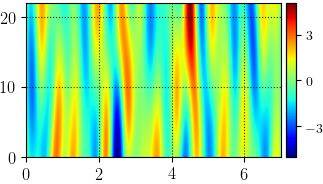
\includegraphics[width=.8\textwidth,height=.2\textheight]{MNG_ppoinitial}
\end{minipage}
\begin{minipage}[height=.2\textheight]{.5\textwidth}
\centering
\small{\texttt{(b)}} \\
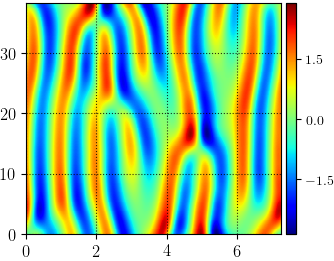
\includegraphics[width=.8\textwidth,height=.3\textheight]{MNG_ppofinal}
\end{minipage}
\begin{minipage}[height=.2\textheight]{.5\textwidth}
\centering
\small{\texttt{(c)}} \\
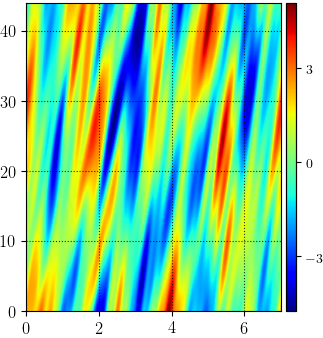
\includegraphics[width=.8\textwidth,height=.39\textheight]{MNG_rpoinitial}
\end{minipage}
\begin{minipage}[height=.2\textheight]{.5\textwidth}
\centering
\small{\texttt{(d)}} \\
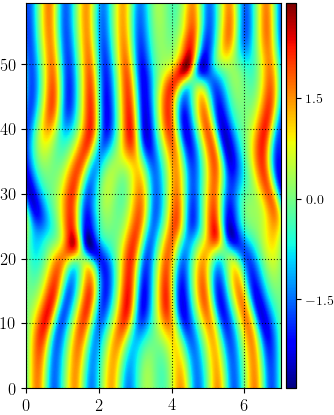
\includegraphics[width=.8\textwidth,height=.48\textheight]{MNG_rpofinal}
\end{minipage}
\caption{ \label{fig:KStrawl}
(a) Initial condition for \twot\ with shift-reflection symmetry, defined on
$\speriod{}=44,\period{}=44$ (fundamental domain). (b) Converged \twot\
resulting from optimization of (a), $\speriod{}\approx 45.58$,$\period{}\approx 76.46$.
(c) Initial condition with spatial translation symmetry (shown in co-moving reference frame),
$\speriod{}=44,\period{}=44$. (d) Converged \twot\ resulting from optimization
of (c), $\speriod{}\approx 44.01$,$\period{}\approx,59.36$,}
\end{figure}

There are alternative methods which we
predict would have greater efficiencies
in terms of convergence.
By taking our library of solutions we can average their
\spt\ Fourier modes to create a template for the ``typical'' spectrum
that different classes of solutions exhibit. There are a number
of things that must be handled carefully, for instance,
for different \spt\ domain sizes the \Fcs\ do not represent
modes with the same frequency so they do not directly map onto
one another. The best way of accounting for the differing domain
sizes is the ``bin'' the frequency data is a method
akin to a histogram. There is another alternative
idea which is hypothetically possible but unclear
whether it is realized.
Our hypothesis is that every \twot\ is comprised of
shadowing of small \spt\ \twots, a topic which we discuss in
much more detail in \refsect{sect:tiles}. If this is
indeed the case then this should be exhibited by
the spectra of the general solution. Therefore,
an additional manner initial conditions could be
created is to take utilize the spectra of just the
tiles.
Looking to the future it has also been put forward that \spt\ methods
will be able to better capitalize on advances in computing, specifically
the increase in number of computational cores\rf{WGBGQ13}.
The idea is that in the future computational speed will not be able
to keep pace with the number of computational cores, and so
one should begin to think in parallel.
Our \spt\ formulation is in the same spirit but unfortunately
we are precluded from the same subdivision that Wang \etal\rf{WGBGQ13} use
because we use periodic boundary conditions. Their idea
is that by subdividing \spt\ domains into subdomains, the equations
being solved locally on each subdomain, in parallel, and then combined
together at their boundaries implicitly. This does not allow for
periodic boundary conditions implying that a \spt\ Fourier basis
is a poor choice. One would want to switch
to either a finite difference scheme or (preferably) a Chebyshev
collocation method in conjunction with new boundary conditions.
On the other side of this discussion, the main
disadvantage of the \spt\ formulation is the increased
number of variables.
To represent the discretization of
a point in the dynamical system's state space we
might use $M$ spatial Fourier modes. The \spt\ equivalent would
be a $N \times M$ \spt\ discretization. In addition, the convergence of
the temporal modes is typically slower than spatial modes because
the time derivatives are of first order. Therefore, not
only must we increase the number of variables by a factor of $N$
but also $N$ will typically be larger than $M$, implying a practical
lower bound of $M^2$ for the number of computational variables. This
quadratic scaling is of course dramatically worse than the $\mathcal{O}(M)$
scaling. The effect of this increase in dimensionality precludes
us from using direct methods such as Newton's method,
as the number of entries of any linearization matrix scales approximately
like $M^4$.



In summary, our \spt\ formulation involves no time integrations and is
thus free of their exponential instabilities. It allows us to
find a large number of numerically accurate \twots\
with comparatively small computational cost.
This allows
us to test our main hypothesis which describes larger \spt\ \twots\
in terms of fundamental ``tiles'' which we shall see in \refsect{sect:tiles}
and \refsect{sect:glue}. Namely, we will demonstrate that it is possible to
take combine subdomains of known solutions to find even more solutions.
These methods exemplify the general idea of a self-sustaining process
in Navier-Stokes flows, in which the general process of sustained
turbulence is described via the interactions of a few fundamental
patterns realized in fluid flows\rf{W97}. By construction their
self-sustaining processes are time dependent; for us however, we
merely are combining patterns and see which are admissible.
Their model is an attempt to describe complex behavior with a
relatively simple model.
%This may be a stretch
This type of modeling can loosely
be interpreted as a dimensional reduction because it attempts
to describe temporal patterns with a small number of ``variables''.
Our \spt\ combinations however do not suffer any reduction in complexity
as we use exact \spt\ solutions of \refeq{e-ks} to describe
all possible patterns.

Know how, does it work

So far we have motivated a {\spt} theory of turbulence
which replaces unstable dynamics with \spt\ patterns.
We formulate these ideas using the \KSe, creating a number of
new numerical techniques in the process.
The following section describes the results of our numerical investigation.

Before we began searching for {\po}s in earnest, we first
tested the efficacy of the {\spt} numerical methods %\MNG{reference section here}
using known {\po}s \rf{SCD07}.
The first test was to find solutions of \refeq{e-Fks} using coarse {\spt} discretizations.
This is important because the main limiting factor
for {\spt} methods is the number of {\cdofs}; the entire orbit must be
kept in the computational memory. It is imperative that we be able to
find {\po}s with coarse resolutions, otherwise the problem is not computationally
feasible unless we consider more advanced computing resources.
Each test performed simply rediscretized a known solution to create an coarse
initial guess, which was then pass to our numerical methods.
In all of the tests we performed, the guess converged to the
``same'' {\po} that it originated from.
Technically, they are not returning
to exactly the same {\po}, but rather, the same family of {\po}s. This
topic arises organically later on when we detail the existence
of continuous families of {\fpo}s, and so we leave the discussion until then.
These tests showed that we could now solve \refeq{e-Fks} with coarse
discretizations, however, using known solutions to perform these tests however
is not very convincing; therefore we then applied
to initial guesses created by adding a substantial amount of noise
to these known {\po}s.

The idea behind this test was simply to see whether or not
the noisy initial guess would converge.
At each field site in the discretization, we drew a value from a
normal distribution with mean zero and whose standard deviation was the
$L_{\infty}$ norm of the {\po}'s field. We only performed a single test
but the results were still  Not only did the
sum of the original field and the noise converge, it converged to the original {\po}
up to translations and small differences in periods.
This exceeded our expectations as the noise was much larger in magnitude
than the original {\po} itself.
Note that we did not include perturbations to the periods but
they remained unconstrained. This test case used a {\po}
with small periods, however, the extent of the noise made us
optimistic that initial guesses of poor quality could be used to find {\po}s.
After these two tests we began the search and collection of {\po}s.
This search applied the methods of \refsect{sect:intro} and
spanned all symmetry types and a range of domain sizes; specifically,
the periods were drawn from the intervals
$L \times T \in [22, 88] \times [20, 200]$.
As a reminder our hypothesis does not require the collection of exceptionally large {\po}s;
they must only be large enough to capture all unique fundamental patterns. If we believed
that this range of periods was insufficient we would have expanded our
search.


Disregarding a few outliers (to be discussed later) the vast majority of {\po}s in this collection
look more or less the same. More precisely, if one were to zoom in on a {\po} and examine
the local features and patterns in a small {\spt} window, neither
the global {\spt} symmetry nor the {\extent} would be ascertainable. This reinforced our belief that {\fpo}s are indeed universal and
can be used to explain all solutions.
The figure %\reffig{fig:waldo}
displays {\po}s of the four different
{\spt} symmetry classes that we considered in our investigation. We believe they are essentially
indistinguishable when only the fundamental domains are plotted (obviously if the symmetry
is visible they can be distinguished from one another).%\MNG{reference figure here}
%\begin{figure}
%\begin{minipage}[height=.05\textheight]{.3\textwidth}
%\centering \small{\texttt{(a)}\\
%\includegraphics[width=.3\textwidth,height=.1\textheight]{MNG_waldo1}
%\end{minipage}
%\begin{minipage}[height=.05\textheight]{.3\textwidth}
%\centering \small{\texttt{(b)}\\
%\includegraphics[width=.4\textwidth,height=.1\textheight]{MNG_waldo2}
%\end{minipage}
%\begin{minipage}[height=.05\textheight]{.3\textwidth}
%\centering \small{\texttt{(c)}\\
%\includegraphics[width=.4\textwidth,height=.1\textheight]{MNG_waldo3}
%\end{minipage}
%\begin{minipage}[height=.05\textheight]{.3\textwidth}
%\centering \small{\texttt{(d)}\\
%\includegraphics[width=.8\textwidth,height=.1\textheight]{MNG_waldo4}
%\end{minipage}
%\caption{ \label{fig:waldo}
%Four {\po}s which demonstrate the ubiquity of patterns irrespective of
%the global symmetry of the housing {\po}.
%}
%\end{figure}
Another means of developing our intuition regarding {\spt} patterns is
to look at the \textit{atypical} patterns of the \KSe.
This classification consists of three main categories: {\po}s which
are `too symmetric', contain `uncommon' patterns, or
which follow an \eqv\ for an extended time.
In dynamical systems context `outliers' is our blanket term for very isolated (unstable) solutions which would hardly ever realized.
Our searches find these outliers
because stability has no affect on the optimization problem.
This implies that our variational method also captures
`rare events', a notably hard problem that has utility in other situations. \MNG{mentioning this worthwhile (or accurate)?}

The usage of `outliers' as opposed to 'isolated' is because solutions exist continuous families
and hence are not `isolated'. Support for our claim that
they are not frequented often is that they are typically found
to exist in the antisymmetric subspace which is very unstable and hence not
visited for long periods of time.  % sources? Lorenz z axis analogy?
Originally we found {\po}s classified as outliers everywhere; but
it may be that they all exist in the antisymmetric subspace. This seems
contradictory if not for a particular computational detail.
It is possible to find antisymmetric solutions
without specifically constraining an initial guess to the antisymmetric subspace.
This is because an antisymmetric {\po}s have the same topology as other {\po}s;
it manifests only as a constraint on the {\Fcs}.
What does this mean? It depends
on the symmetries being compared but here are two examples. In figure %\MNG{figure reference here}
demonstrates a {\po} found with no imposed symmetry.
Another possibility occurs with shift-reflection invariant {\po}s. Due to
the nature of the constraints on the {\Fcs}, imposing shift-reflection symmetry
can also find even multiples of prime periods of antisymmetric {\po}s;
i.e. two, four, etc. repeats of antisymmetric solutions in time.
These aren't just assumptions either; these solutions can actually be converged to the
antisymmetric subspace if their reflection axes are restored, as seen in {}.
This demonstrates that {\po}s with discrete symmetries are simply special representatives
of their group orbit produced via translations.
This would have never been realized in the dynamical
systems context due to the instability of the antisymmetric subspace.%\MNG{is this actually a new revelation?}
%The solution %\reffig{rposlant}
%demonstrates a behavior that is not particularly common on smaller domain sizes.
%\subsubsection{Analysis of the library}
%examples of initial conditions and their converged results.
%examples depicting similar structures regardless of symmetry
%examples demonstrating repeats of the structures after a prescribed length
%examples of similar yet deformed structures / the structure's scales.
%\subsubsection{Outliers}
%Under resolved solutions
%Large equilibria solutions?

We have displayed {\po}s that we consider to be both typical and atypical.
Our intuition evolved to the point where we could identify {\fpo} candidates.
The notable property of these candidates is that they not only occur frequently throughout the
{\po} collection; they also occur frequently within individual {\po}s.
To further motivate the existence of
{\fpo}s as well as some initial guesses, we direct the reader to %\MNG{figure reference here}
where a very large time integrated trajectory (aperiodic in time)
is displayed. Notable in this figure is the {\spt}
frequency with which a single pattern occurs.

The first guess was the {\wiggle} which appears in% \MNG{figure reference here}
It very distinctly repeats twice with respect to time in
and is relatively small in spatial scale, containing only two notable wavelengths.

This was the inaugural search for a {\fpo} and so extra
care was taken in the clipping process \refsect{sect:intro}.
In this instance the clipping was done iteratively, finding
a sequence of progressively smaller {\po}s each of which contained the {\fpo}.
We now know that it is was possible to clip and converge {\fpo}s in a single clipping,
but this example is kept in its entirety to demonstrate additional utility.

The results of the {\wiggle} search are as displayed in %\MNG{figure reference here}
The final result was an antisymmetric {\fpo} whose velocity field on
the fundamental domain consisted of a wavelength or streak ``wiggling'', hence the name.
To check our work, comparison of this pattern with our {\po} collection was made.
While the {\wiggle} was converged in the antisymmetric subspace, the
pattern most often as a pair of wiggles.
As previously mentioned in the discussed of ``outlier'' {\po}s, the antisymmetric {\wiggle}
should be viewed as a special case of the continuous family of {\wiggle} solutions as
this case will never appear in actuality.

The collection of the {\wiggle} not only provided us with our first {\fpo} but also
provided us with an obvious guess for the second {\fpo}. If we look back
at the iterative clipping procedure that we just performed, %\MNG{figure reference here}
we see that the {\wiggle} is spatially adjacent to an additional,
single wavelength {\eqv}. %\MNG{figure reference here}
By appealing to the notion of {\spt} {\symbolic} we postulated that
this {\eqv} would be our second {\fpo}. Indeed, by clipping this
single wavelength {\eqv} from the original {\po} another {\fpo} was found,
which we now refer to as the {\streak}.

At this point we knew that our library was yet incomplete as we had not
captured the pattern emphasized in %large cutouts.
This pattern, now named the {\defect}, captures two very important physical processes (they
could be interpreted as two sides of the same coin, really). First, two spatially adjacent
wavelengths merge into a single wavelength. In the gap in space-time left behind by this
merger, a new wavelength emerges. The result is a new pair of wavelengths which
exhibit an approximate phase difference of a
half wavelength with the original pair (approximately a quarter of
the spatial period).
This {\defect} epitomizes two very important mechanisms of the \KSe:
fluctuations in global wavelength count and local spatial drift velocity.
Neither the {\streak} nor the {\wiggle} can account for
these behaviors, highlighting the importance of the {\defect}.
The actual search for the {\defect} was quite challenging relative to the other
{\fpo}s. Due to the spatial
shift it should be no surprise that the {\fpo} was assumed to be a {\rpo}.
Locating the {\defect} proved to be much more difficult than both the {\wiggle}
and {\streak}, in part due to the extra {\cdof} from the spatial shift.


\MNGedit{After our first search concluded, we believed that there were four unique {\fpo}s.
Upon further review two of these four {\fpo}s looked quite similar visually, leading us
to believe that they were related. This was verified by pseudo-arclength continuation using
the spatial period as the parameter. Continuation was performed until the spatial periods
of this {\fpo} pair were the same. By fixing the phases of the
{\Fcs} it is quite clear that these {\fpo}s are equivalent.
This brought about a revelation regarding
{\fpo}s that had been previously glossed over;
{\fpo}s exist in continuous families. In hindsight it could not have been
any other way. Shadowing by {\fpo}s is not an exact process;
clippings from larger trajectories always look similar but not identical. This
property is precisely captured by continuous families: which are
infinite sets of solutions related by continuous deformations.}

From a dynamical systems perspective
this is not shocking nor new as previous bifurcation analyses
track different branches of {\po}s.
The main effect of these families is that our {\symbolic}
now consists of a ``rubbery'' continuous alphabet, as opposed to a static discrete one.
For each symbol in any {\spt} {block}, the symbol now represents a continuous
family of {\fpo}s. To best illustrate the effect of this,
we delve into the continuous family of the {\defect}.
We display the numerical continuation of the defect as a
function of the spatial period noting
that there are other manners with which {\po}s can be continued. A collection of representatives
are displayed in {}. The main result of the investigation is
that the family is perhaps more properly parameterized
by the spatial shift parameter.
% more on defect family.

It might be accurate to say that all {\po}s
exist in continuous families \emph{because} {\fpo}s exist in
continuous families. This initially betrayed our intuition; in hyperbolic systems, {\po}s are
isolated solutions by virtue of their unstable manifolds. In any case each continuous
family seems to exist on a finite interval of spatial periods, punctuated by what are
presumed to be bifurcations. It could be that this assumption is incorrect and that we
are failing to track the correct branch of the solutions.
Exploration of the {\fpo} continuous families reduced the alphabet
to three. To reiterate; there may only be three {\fpo}s
needed to describe all solutions of the {\KSe}.

It is absolutely essential to understand the notion of continuous families of {\fpo}s
and so we summarize it here before moving on to the description of gluing results. We postulated
and then found a collection of {\fpo}s whose existence can ostensibly describe all solutions.
We believe that this collection consists of three unique {\fpo} continuous families.
We currently do not have a clear manner with which to develop a {\spt} {\symbolic}.
To begin the investigation, however, we can test our ideas by creating
{\spt} combinations of {\fpo}s. This is the aforementioned gluing method,
whose results shall now be described.


First as a proof of concept we reproduce a known solution by combining many small,
custom tailored components. Next, we demonstrate how to glue known {\po}s along a single spacetime dimension: either time or space.
Lastly, we glue {\spt} combinations of {\fpo}s to find {\po}s.
The first question we aimed to answer was ``Can a known solution be reproduced by combining many different clippings from
other solutions?''.  This is demonstrated in %reffig{}.
where a handmade {\spt} combination was used to create an initial guess for a specific {\po} which
is known to exist.

The resultant {\po} is essentially a reproduction of the target up to continuous family considerations. This prototype of the gluing method was developed concurrently with the search
for {\fpo}s. In this case the constituent pieces are not converged {\fpo}s but merely clippings from {\po}s not including the target. The success of this trial gave credence to the argument for {\po}s
existing as collections of {\fpo}s.
While this result was very encouraging it was also somewhat contrived.
The initial guess was hand tailored to be a rough approximation to the
targeted {\po}. Therefore we did not know whether this result would generalize.
The next step was to implement unsupervised gluing along a single continuous dimension.
In this context ``unsupervised'' implieds that the only decision
that is made is which {\po}s to glue together.
We focus on only gluing one pair of {\po}s at a time but also demonstrate
that this process can be applied iteratively.

We begin by temporally gluing {\po}s with small spatial periods,
a familiar notion to those cognizant of periodic orbit theory. Our computation
is completely different however as the spatial periods are allowed to differ
as well as freely vary.
Upon success we were able to find {\po}s with large temporal periods.
For instance, in %reffig
the final converged {\po} is a shift-reflection invariant orbit whose fundamental domain
has period $386.088... / 2$. Similarly in %reffig
is an examples of a converged {\rpo} with time period $231.419...$. These periods
are what we would expect if the gluing was properly functioning, as they are
approximately the sum of the periods of the original {\po}s.
These {\po}s are much longer than anything we have seen
in the literature which again exemplifies how robust
our {\spt} methods are.

In line with our identical treatment of space and time we also glue {\po}s spatially.
The figures %reffig reffig
show exactly this where the original {\po}s, their gluing, and the resultant {\po} are shown.
In %reffig{MNGppo12spaceglue}
two {\po}s with shift-reflection symmetry were chosen to be glued in space.

Much like the clipping process we can also iteratively glue to create a sequence of
progressively larger {\po}s. To demonstrate this, we glue the result
from the previous example to yet another {\po} with shift-reflection symmetry. Originally
the choice was made to only glue in a symmetry preserving manner; shift-reflection symmetric
orbits were only glued to other shift-reflection symmetric orbits, and the result was
also constrained to have shift-reflection symmetry. It was realized that there
was no real motivation behind this choice and so this requirement was removed, such that
it is not applied in the next section when discussing gluing {\fpo}s together.


Showing that we can both glue in space and time we proceed to
the ultimate method: gluing {\spt} combinations of {\fpo}s.
To review our motivation, let us again explain the process in terms of {\symbolic}.
The initial guesses can be thought of as symbolic blocks, where each symbol
is representative of a {\fpo}'s continuous family. Quite literally, the symbols are replaced
by these {\fpo}s to construct an initial guess; an approximation to a possible {\po}.
We elect to use a static set of
representative {\fpo}s for each of these substitutions with no motivation other
than simplicity. Specifically: the {\defect},
{\wiggle}, and {\streak} displayed in %reffig final tiles.

To deem each gluing as a success, they must satisfy a {\symbolic} requirement
in addition to numerical convergence. Namely, the initial guesses must converge
to a {\po} which has the ``correct'' symbolic representation.
That is, it must be contain the {\fpo}s which befits its construction.
Yet again, however, we are forced to rely upon visual inspection to validate our results.
First, we provide examples which we claim are successful under our new requirement.
Next, are examples of numerical success but ``symbolic failure''.
The existence of this class of outcomes, in combination with our lack of verification of results,
contributes to the challenge of making the {\symbolic}. Specifically,
this prevents us from determining the correct grammar of
the {\symbolic}; the rules which dictate whether each {block} is admissible {\po} or not.

In summary we have shown that it is possible to use our techniques to find {\po}s by construction,
clipping and gluing. In essence
clipping and gluing are inverses of one another, however, gluing is
typically more difficult than clipping due to the inherent differences in complexity. In practice,
we usual clip in a single step but glue iteratively.
Currently we have a very surface level method and there are currently many unknowns in regards to best practices. Essentially we have made the simplest choices which result in the gluing method to be
numerically well defined. While these results are very informative they leave us with more open
questions than we started with \refsect{sect:future}. The future is bright, however, as the number of potential improvements seems to be limited only by our creativity.

Discounting the time it took to produce the codes used for
the computations, it did not take much effort to complete the
collection of \twots. This search was performed over intermediately
sized domains and all symmetry types.

The first test of the ideas was to converge coarse discretizations
of known solutions. When converged using shooting type methods, the
number of discrete time steps numbers in the thousands. When converged
using other variational techniques such as the Newton descent method, \rf{LanThesis}
mentions using upwards of 512 to 1024 discrete time points. Meanwhile, the method
proposed here can converge solutions on very coarse discretizations orders of magnitude smaller
than these other methods. This is slightly disingenuous as the shooting type method does
not require all of the points to be maintained in memory; this is merely an
argument that the memory requirements for \spt\ methods do not need to be nearly
as large as one might imagine. This reduces even further if imposing discrete symmetries;
a common occurrence in flows such as pipe and and plane Couette flows \rf{GHWC07}.
The familiarity with finite difference methods leads to another foreseeable counter argument;
coarse discretization which do not resolve the appropriate physical scales lead to nonsensical
solutions, regardless of whether or not they converge. This is exactly the case; if the problem
were to be composed of finite differences in physical space. The coarse discretization in
Fourier space is sufficient to resolve all physically relevant modes a quick visual inspection is
typically sufficient; this can be done by interpolating a finer grid via zero padding.
If skepticism remains an alternative would be to alternative between zero padding and converging.
This works but it will change the \spt\ dimensions if they remain free parameters and so
the lattice dimension is best increased in small increments. It is possible to perform
this type of extension to a very large dimension but it is very hard to decrease the error;
we recommend using this as an error density such that the absolute tolerance becomes
$NM \cdot 10^{-15}$ instead of $10^{-15}$. This remains a qualitative value but there
is evidence that the tolerance need not be machine precision for the calculations at least
in the spatiotemporal setting which lacks dynamical instability. As a test of practicality of
this bound a numerical experiment was ran which attempted to converge a known solution using
a discretization which dwarfed the original. After a finite number of gradient descent steps
a spatial strip was taken from the approximate solution and integrated in time to test whether
or not this would reproduce the solution. A successful test increased a \spt\ discretization
of size $[64, 32]$ to $[4096, 512]$. Not many tests were run so this could be an indication
of sampling bias, but it was informative at least in regards to whether or not this formulation
could work for higher dimensional equations.

Once this preliminary testing was completed, we started trawling the solution space
for \twots. The parameter ranges employed for the search varied, but the typical ranges were
$L \in [22, 66]$, $T \in [20, 180]$. The typical lattice dimensions over these ranges
were $N\times M \in [32, 128] \times [32, 64]$.

The typical pattern for finding a solution was as follows. An initial field with very
large magnitude of the cost function, upwards of $\approx 10^{10}$, is annealed by the descent
algorithm.
This uses the method described in %\refsect{how}


 typically ending at the maximum step limit instead of the numerical
tolerance. The annealed approximation is then passed
to the least-squares backtracking algorithm. The damping
typically starts high until the the approximation nears a \twot with
the last few steps typically being undamped.
``Rough patches'' are also common during the least-squares
backtracking routine; this term represents local regions where the damping increases
presumeably due to increased curvature of the cost function.

The computation times to find solutions ranged from seconds to tens of minutes, depending
heavily on the dimensionality of the discretization. The solutions which converged the fastest always resulted
from smaller solutions which did not take much time at all to complete the descent algorithm;
essentially they would be immediately passed to the least-squares algorithm.


\begin{figure}
\begin{minipage}[height=.05\textheight]{.5\textwidth}
\centering
\small{\texttt{(a)}} \\
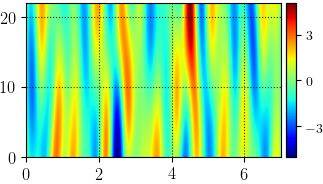
\includegraphics[width=.8\textwidth,height=.2\textheight]{MNG_ppoinitial}
\end{minipage}
\begin{minipage}[height=.2\textheight]{.5\textwidth}
\centering
\small{\texttt{(b)}} \\
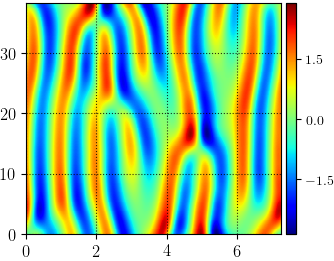
\includegraphics[width=.8\textwidth,height=.3\textheight]{MNG_ppofinal}
\end{minipage}

\caption{ \label{fig:ppo1}
(a) Initial condition for \twot\ with shift-reflection symmetry, defined on
$\speriod{}=44,\period{}=44$ (fundamental domain). (b) Converged \twot\
resulting from optimization of (a), $\speriod{}= 45.58\dots$,$\period{}= 76.46\dots$.
(c) Initial condition with spatial translation symmetry (shown in co-moving reference frame),
$\speriod{}=44,\period{}=44$. (d) Converged \twot\ resulting from optimization
of (c), $\speriod{} = 44.01\dots$,$\period{}=59.36\dots$,}
\end{figure}

In \reffigs{fig:ppo1, fig:rpo1} we demonstrate a

\begin{figure}
\begin{minipage}[height=.05\textheight]{.5\textwidth}
\centering
\small{\texttt{(a)}} \\
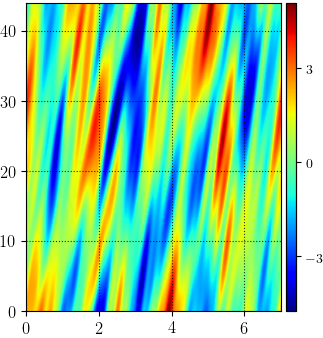
\includegraphics[width=.8\textwidth,height=.39\textheight]{MNG_rpoinitial}
\end{minipage}
\begin{minipage}[height=.2\textheight]{.5\textwidth}
\centering
\small{\texttt{(b)}} \\
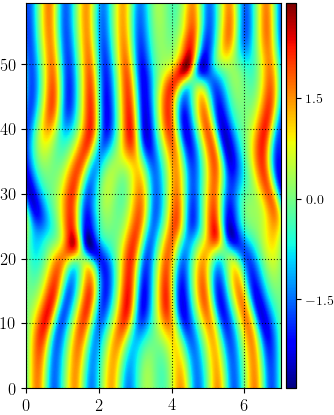
\includegraphics[width=.8\textwidth,height=.48\textheight]{MNG_rpofinal}
\end{minipage}
\caption{ \label{fig:rpo1}
(a) Initial condition with spatial translation symmetry
(displayed in co-moving reference frame),
$\speriod{}=44,\period{}=44$. (b) Converged \twot\ resulting from optimization
of (c), $\speriod{} = 44.01\dots$,$\period{}=59.36\dots$,}
\end{figure}

%more examples, anti, eqva, different kinds of initial condition generation?

%Tiles
After examination of our library of solutions we determined that there are
only a small number of fundamental patterns. We have tentatively named
these patterns after the basic physical processes they represent.
The first tile is actually defined with $T=0$

They can be described by the
following physical processes.


Upon convergence of the
guesses for these tiles, this number reduced even further upon realization
that some of the guesses belong to the same continuous family.

Despite our best efforts to determine the opposite, no continuous symmetry
was found that explains these continuous families of tiles.

The interpretation of these families is that instead of having a unique, finite set of tiles
we instead

The most frequent patterns, that is, those which are presumably the best tile
candidates are relatively simple to describe in terms of physical processes.
This description is best carried out in the context of spatial waves present
in each solution. The natural length scale of the equations

The most unstable wavelength, however, seems to mediate the interaction between these
waves.
The ``most'' fundamental of the tiles is what we have denoted as the streak tile.


Our
naming convention appeals to similar shapes witnessed in fluid simulations.
It has been argued that the natural length scale of the problem is the wavelength
corresponding to the most unstable mode. Visual inspection of arbitrary
solutions shows a slightly more detailed story best described as a tug-of-war between two
different length scales. The most unstable wavelength results from the linearized
spectrum; while informative it does not encapsulate the full story. Luckily the
tiles The number of pronounced (amplitude above a threshold)
wavelengths varies over time, seemingly oscillating between these two different scales.

The transition to the
most unstable wavelength seems to be a transient phenomenon that accounts for
the destruction of wavelengths via collision. This is not simply linear
superposition of waves but the linear affects can be
The equilibria



\MNGedit{
Specifically, we need a collection {\po}s
defined over a range of spatial and temporal periods. This is achieved by creating
initial guesses whose periods exist on some finite range of values.
Once a library of {\po}s has been created, we identify the most frequently
occurring patterns which, by our claim,
are regions of spacetime shadowed by {\fpo}s. Once a handful of {\fpo}
candidates are decided upon, the next step in the {\spt} pipeline is to convert
them into initial guesses; we do so with a technique we call `clipping'.}
\MNGedit{2020-05-15}{
The search for {\po}s combines the initial guess creation of \refsect{sect:guesses}
with the numerical optimization methods \refsect{sect:descent}, \refsect{sect:leastsquares}.
For the numerical methods, a handful of parameters are required such as the step limit
and tolerance. Our typical choices, noting that they are likely suboptimal, are as follows:
the tolerance of the cost function for the gradient descent was $J = 10^{-4}$
and the step limit was set to a multiple of the dimension, either $16NM$ or $32NM$.
This means that if either \refeq{e-cost} $J < 10^{-4}$ or the step limit
is reached, then the descent method terminates, and the guess is passed to the
least-squares implementation.
The ``heavy lifting'' was delegated to the least-squares method
with backtracking. The threshold for termination was originally set to double
floating point precision but over time this was relaxed to incorporate the {\cdof}, i.e.
the current tolerance is on the order of $(NM)*10^{-15}$; and the step limit, $500$.
For those familiar with Newton methods, this number of steps appears like overkill at first, but the
allowance of backtracking negatively impacts the rate of convergence.
    } 